\section{Procedure}

In the procedure section a heuristic algorithm is provided for the Minimum Height Problem. Recall that the 
Minimum Height Problem asks, given some $\pi$ is there an algorithm for creating a minimal ladder 
from $MinL\{\pi\}$? Before providing the heuristic algorithm, it must be stated that there is an exact  
procedure to generate a minimal ladder from each $MinL\{\pi\}$ from $MinL\{\pi_{N}\}$. In the introduction of this chapter, there 
is a description of a removal sequence of bars from the minimal ladder for the reverse permutation of order $N$, resulting in one  
minimal ladder for each $MinL\{\pi\}$ from $MinL\{\pi_{N}\}$. However, this method for creating a minimal ladder is not efficient. 
Using this method on some arbitrary permutation $\pi$ would first require creating the root ladder for the reverse 
permutation of order $N$, then swapping every other route in the root ladder to create a minimal ladder
for the reverse permutation. Once the swapping is completed, each bar in the minimal ladder for the reverse permutation that 
does not correspond to the inversion set of $\pi$ would need to be removed from the minimal ladder of the reverse permutation. 
The resulting ladder is a minimal ladder from $MinL\{\pi\}$. To see an example of the exact procedure 
for creating a minimal ladder, given some arbitrary $\pi$ of order $N$ please refer to Fig. \ref{Fig:ExactProcedure}.

\begin{figure}[!htp]
    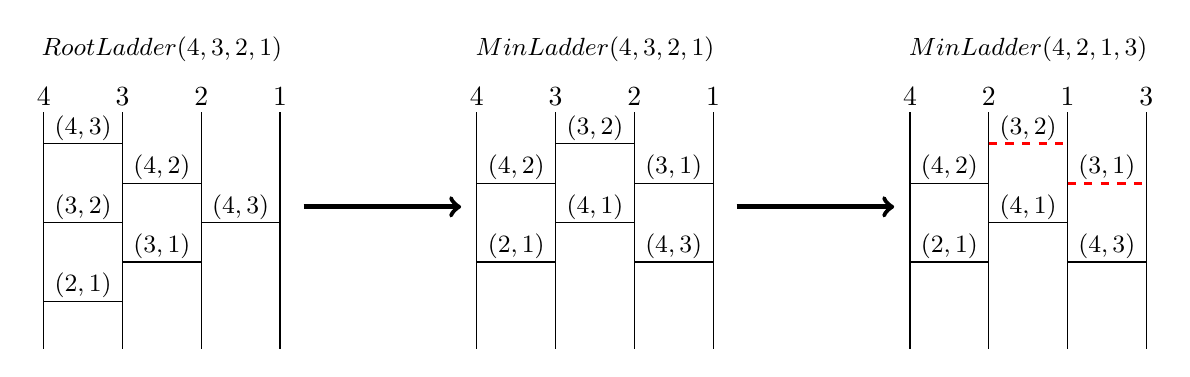
\begin{tikzpicture}
        
        \node at(0, 3.2){4};
        \node at(1, 3.2){3};
        \node at(2, 3.2){2};
        \node at(3, 3.2){1};
        \node at(1.5, 3.8){\small{$Root Ladder(4,3,2,1)$}};

        \node at(.5, 2.8){\small{$(4,3)$}};
        \node at(1.5, 2.3){\small{$(4,2)$}};
        \node at(2.5, 1.8){\small{$(4,3)$}};
        \node at(.5, 1.8){\small{$(3,2)$}};
        \node at(1.5, 1.3){\small{$(3,1)$}};
        \node at(.5, .8){\small{$(2,1)$}};
        \draw(0, 0) to (0, 3);
            \draw(0, 2.6) to (1, 2.6);
            \draw(1, 2.1) to (2, 2.1);
            \draw(2, 1.6) to (3, 1.6);
        \draw(1, 0) to (1, 3);
            \draw(0, 1.6) to (1, 1.6);
            \draw(1, 1.1) to (2, 1.1);
        \draw(2, 0) to (2, 3);
            \draw(0, .6) to (1, .6);
        \draw(3, 0) to (3, 3);

        \draw[->, line width=.6mm](3.3, 1.8) to (5.3, 1.8);

          
        \node at(5.5, 3.2){4};
        \node at(6.5, 3.2){3};
        \node at(7.5, 3.2){2};
        \node at(8.5, 3.2){1};
        \node at(7, 3.8){\small{$Min Ladder(4,3,2,1)$}};


        \draw(5.5, 0) to (5.5, 3);
            \draw(5.5, 2.1) to (6.5, 2.1);
            \draw(6.5, 1.6) to (7.5, 1.6);
            \draw(7.5, 1.1) to (8.5, 1.1);
        \draw(6.5, 0) to (6.5, 3);
            \draw(6.5, 2.6) to (7.5, 2.6);
            \draw(7.5, 2.1) to (8.5, 2.1);
        \draw(7.5, 0) to (7.5, 3);
            \draw(5.5, 1.1) to (6.5, 1.1);
        \draw(8.5, 0) to (8.5, 3);

        \node at(7, 2.8){\small{$(3,2)$}};
        \node at(8, 2.3){\small{$(3,1)$}};
        \node at(6, 2.3){\small{$(4,2)$}};
        \node at(7, 1.8){\small{$(4,1)$}};
        \node at(8, 1.3){\small{$(4,3)$}};
        \node at(6, 1.3){\small{$(2,1)$}};

        \draw[->, line width=.6mm](8.8, 1.8) to (10.8, 1.8);

        
        \node at(11, 3.2){4};
        \node at(12, 3.2){2};
        \node at(13, 3.2){1};
        \node at(14, 3.2){3};
        \node at(12.5, 3.8){\small{$Min Ladder(4,2,1,3)$}};

        \draw(11, 0) to (11, 3);
            \draw(11, 2.1) to (12, 2.1);
            \draw(12, 1.6) to (13, 1.6);
            \draw(13, 1.1) to (14, 1.1);
        \draw(12, 0) to (12, 3);
            \draw[red, dashed, line width = .4mm](12, 2.6) to (13, 2.6);
            \draw[red, dashed, line width = .4mm](13, 2.1) to (14, 2.1);
        \draw(13, 0) to (13, 3);
            \draw(11, 1.1) to (12, 1.1);
        \draw(14, 0) to (14, 3);

        
        \node at(12.5, 2.8){\small{$(3,2)$}};
        \node at(13.5, 2.3){\small{$(3,1)$}};
        \node at(11.5, 2.3){\small{$(4,2)$}};
        \node at(12.5, 1.8){\small{$(4,1)$}};
        \node at(13.5, 1.3){\small{$(4,3)$}};
        \node at(11.5, 1.3){\small{$(2,1)$}};


    \end{tikzpicture}
    \caption{Given $\pi=(4,2,1,3)$, the exact procedure first creates the root ladder for $(4,3,2,1)$ then creates a min ladder for $(4,3,2,1)$ then removes bars to create a min ladder for $(4,2,1,3)$}
    \label{Fig:ExactProcedure}
\end{figure}


\begin{algorithm}
        \begin{algorithmic}[1]
            \Function{HeuristicMinLadder}{$Ladder[N][N-1]$, $\pi$, $N$, $Row \gets 0$}
                \If{\small{$Sorted(\pi)$}}
                    \State \small{return}
                \EndIf
                \If{\small{$Row = 0$}}
                    \State \small{$\pi,Ladder \gets PreProcessRow(Ladder, \pi)$}
                    \State \small{$HeuristicMinLadder(Ladder, \pi, N, Row \gets Row+1)$}
                \Else
                    \For{\small{$i \gets 0, i < N, i \gets i+1$}}
                        \If{\small{$\pi_{i}>\pi_{i+1}$}} 
                            \State \small{$Swap(\pi{i}, \pi_{i+1})$}
                            \State \small{$Ladder[Row][i] \gets 1$}
                        \EndIf
                    \EndFor
                    \State \small{$HEURISTICMINLADDER(Ladder, \pi, N, Row \gets  Row+1)$}
                \EndIf


            \EndFunction


        \end{algorithmic}

         \begin{algorithmic}[1]
            \Function{PreProcessRowZero}{$Ladder[N][N-1]$, $\pi$, $N$}
                \State \small{$\pi' \gets \pi$}
                \State \small{For each even lengthed deacreasing substring in $\pi$, swap all adjacent inversions in the decreasing substring in $\pi$.}
                \State \small{$\pi'' \gets \pi$}
                \State \small{$pi''' \gets \pi$}
                \State \small{For each odd lengthed decreasing subsrting in $\pi'$, swap all the adjacent elements belonging to the same decreasing substring 
                in $\pi''$, going left to right.}
                \State \small{For each odd lengthed decreasing subsrtiing in $\pi'$, swap all adjacent elements belonging to the same decreasing substring 
                in $\pi'''$ going right to left.}
                \If{\small{$\pi''$ and $\pi'''$ have the same number of odd lengthed decreasing substrings}}
                    \State return $\pi'''$
                
                \Else 
                    \State \small{return $Min(\pi'',\pi''')$ where $Min$ returns the permutation with the minimal number of odd lengthed decreasing substrings.}
                \EndIf

            \EndFunction
        
        \end{algorithmic} 
        \caption{Heuristic Algorithm for creating a Minimal Ladder}
        \label{Algo:heuristic}
\end{algorithm}
